\section{Methodology \& Computer Vision Algorithm}
\label{sec:method}
\subsection{Methodology}
\label{subsec:method}
1. Research datasets to use \cite{YOLOpaper2}
2. Research models to use 
3. Selected COCO Dataset and YOLOv6 \cite{YOLOpaper1} model
4. Train that model to recognize humans in an image \cite{YOLO}
5. Test the trained model to recognize the students in the class from images taken by group members

The model will be trained using a portion of the Microsoft COCO dataset. The model will be used to recognize the students in the class, apply bounding boxes around the students recognized and sum up the number of bounding boxes to get a total count of students in that image. As an addition, we noticed that we were not able to capture an entire classroom in 1 image from the front, we have also presented an option to the instructor to take numerous pictures and stitch them together into 1 image and then do a total sum of students found.\\ 

\subsection{Computer Vision Algorithm}
\label{subsec:Computer Vision Algorithm - YOLOv6}
We chose to use the YOLO (You Only Look Once) \cite{YOLO} model. YOLO uses a single neural network to simultaneously predict bounding boxes and class probabilities, making it ideal for applications demanding instantaneous detection such as our project. \\
Since it's introduction in 2016, YOLO has undergone significant improvements. YOLOv2 was released in 2017, YOLOv3 in 2018, etc. these numerous iteration included refined accuracy and speed, and incorporated multiple scales for object detection \cite{YOLO4}. YOLO showcases the hallmarks of a good model due to it's advancements that continue to propel it to the forefront of real-time object detection technology. This lengthy history also makes it an ideal choice to use for our project since we can easily find numerous resources and blog posts referring this model.\cite{YOLO5}\\
% Diagram of the system%
\begin{figure}[h]
    \centering
    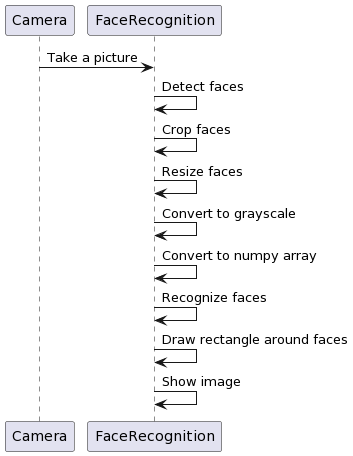
\includegraphics[width=0.5\textwidth]{images/Diagram-1.png}
    \caption{Flowchart of the system}
    \label{fig:flowchart}
\end{figure}

%-------------------------------------------------------------------------
